\documentclass[11pt,a4paper]{article}
\usepackage[margin=2.5cm]{geometry}
\usepackage{amsmath,amssymb}
\usepackage{booktabs}
\usepackage{siunitx}
\usepackage[hidelinks]{hyperref}
\usepackage{microtype}
\usepackage{graphicx}
\usepackage{tikz}
\usetikzlibrary{arrows.meta,positioning}
\definecolor{accent}{HTML}{2A78D6}
\definecolor{edge}{HTML}{898781}

\newcommand{\koff}{k_{\mathrm{off}}}
\newcommand{\poff}{p_{\mathrm{off}}}
\newcommand{\pb}{p_{\mathrm{b}}}
\newcommand{\npar}{\nu_\parallel}
\newcommand{\nperp}{\nu_\perp}

\title{From F\"orster transfer to directed percolation:\\
the photoswitching dye lattice as a contact process}
\author{Calvin Sabastian Tanzil}
\date{Draft, 15 October 2026}

\begin{document}
\maketitle

\begin{abstract}
A lattice of photoswitching Cy5 dyes, in which an ON dye can return a dark
neighbour to ON by energy transfer, realises a contact process. We derive the
coupling between two dyes from F\"orster theory and the dye's switching
photophysics, show that the resulting dynamics satisfies the conditions of the
directed-percolation (DP) conjecture, and treat the three experimental
imperfections --- spontaneous recovery, photobleaching and quenched disorder ---
as perturbations of the DP fixed point. Each perturbation gives a crossover time
that scales as a power of its strength. The predicted crossover times agree
with exact stochastic simulations to within about 20\,\%. The scaling arguments
are ours; the DP exponents and the Harris criterion are standard.
\end{abstract}

\section{Microscopic model}

Each dye $i$ is in one of three states: ON ($n_i=1$), dark but recoverable
($n_i=0$), or bleached. An ON dye is excited at rate $k_{\mathrm{exc}}$,
proportional to the laser irradiance. From its excited singlet state S$_1$ the
dye can
\begin{enumerate}
  \item relax to the ground state, by fluorescence or internal conversion (total
  rate $k_D=1/\tau_D$);
  \item enter the long-lived dark state, by photoinduced electron transfer from
  thiolate, either directly or via the triplet; we write the probability per
  excitation as $\poff$;
  \item transfer its energy to a dark neighbour $j$ at the F\"orster rate
  \begin{equation}
    k_T(d_{ij}) = k_D\left(\frac{R_0}{d_{ij}}\right)^{6},
    \qquad
    R_0^6 = \frac{9\ln 10\,\kappa^2 \Phi_D}{128\pi^5 n^4 N_A} J_{\mathrm{off}},
    \label{eq:forster}
  \end{equation}
  where $J_{\mathrm{off}}$ is the overlap of the ON-dye emission with the
  dark-state absorption. A transfer returns $j$ to ON with probability $\eta$.
\end{enumerate}
Bleaching ends an ON period with probability $\pb$. Figure~\ref{fig:states}
summarises the rules.

\begin{figure}[h]
\centering
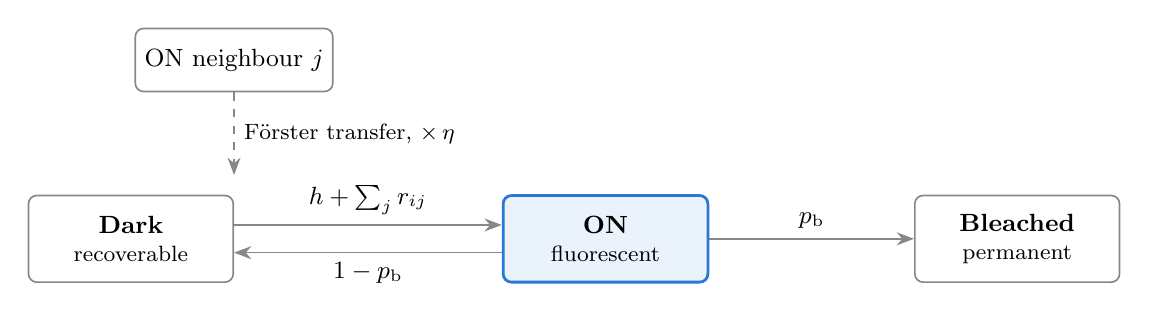
\begin{tikzpicture}[>={Stealth[length=2.2mm]}, every node/.style={font=\small},
  st/.style={draw=edge, rounded corners=3pt, minimum width=2.6cm, minimum height=1.1cm, align=center, line width=0.6pt}]
  \node[st] (dark) {\textbf{Dark}\\[-1pt]{\footnotesize recoverable}};
  \node[st, draw=accent, fill=accent!10, line width=1pt, right=3.4cm of dark] (on) {\textbf{ON}\\[-1pt]{\footnotesize fluorescent}};
  \node[st, right=2.6cm of on] (bl) {\textbf{Bleached}\\[-1pt]{\footnotesize permanent}};
  \node[st, minimum width=2.4cm, minimum height=0.8cm, above=1.3cm of dark.north east, anchor=south] (nb) {ON neighbour $j$};
  \draw[->, edge, line width=0.6pt] ([yshift=5pt]dark.east) -- node[above, text=black] {$h+\sum_j r_{ij}$} ([yshift=5pt]on.west);
  \draw[->, edge, line width=0.6pt] ([yshift=-5pt]on.west) -- node[below, text=black] {$1-\pb$} ([yshift=-5pt]dark.west -| dark.east);
  \draw[->, edge, line width=0.6pt] (on) -- node[above, text=black] {$\pb$} (bl);
  \draw[->, edge, dashed, line width=0.6pt] (nb.south) -- node[right, text=black, font=\footnotesize] {F\"orster transfer, $\times\,\eta$} ++(0,-1.05);
\end{tikzpicture}
\caption{The dye rule, with rates in units of the off rate $\koff$. Only the
recovery rate depends on the neighbours; $r_{ij}$ comes from F\"orster transfer
(Eq.~\ref{eq:d0}).}
\label{fig:states}
\end{figure}

\paragraph{Rates.} Let $E_{ij}=k_T(d_{ij})/(k_D+\sum_l k_T(d_{il}))$ be the
fraction of $i$'s excitations transferred to $j$. The rate at which ON dye $i$
wakes dark dye $j$, and the rate at which $i$ itself goes dark, are
\begin{equation}
  \lambda_{ij} = k_{\mathrm{exc}}\,\eta\,E_{ij},
  \qquad
  \koff = k_{\mathrm{exc}}\,\poff .
\end{equation}
Both are proportional to $k_{\mathrm{exc}}$, so the excitation rate sets only the
clock. Measuring time in ON lifetimes, $t\to\koff t$, the only coupling is
\begin{equation}
  r_{ij} = \frac{\lambda_{ij}}{\koff} = \frac{\eta}{\poff}\,E_{ij}.
\end{equation}
In the weak-transfer limit, $E_{ij}\approx (R_0/d_{ij})^6$, this becomes
\begin{equation}
  \boxed{\;r(d) = \left(\frac{d_0}{d}\right)^{6},
  \qquad
  d_0 = R_0\left(\frac{\eta}{\poff}\right)^{1/6}\;}
  \label{eq:d0}
\end{equation}
For a pair, the hand-over probability (an ON dye wakes its dark neighbour before
going dark) is $B=r/(1+r)$.

\paragraph{Numbers.} With the Cy5 spectra and constants of Ebert, Sauer and
Doose (2026), $R_0=\SI{4.29}{nm}$, $\eta=10^{-4}$ and
$\poff=6.5\times10^{-6}$ (\SI{100}{mM} MEA, pH 7.5), Eq.~\eqref{eq:d0} gives
$d_0=\SI{6.77}{nm}$, in agreement with the full model's $\SI{6.74}{nm}$. If the
transferred photon wakes the dark dye no more efficiently than a directly
absorbed one ($\eta\approx 2\times10^{-7}$), then $d_0=\SI{2.38}{nm}$.

\paragraph{Sensitivity.} Eq.~\eqref{eq:d0} has two useful consequences. A
critical coupling $r_c$ fixes a critical spacing
\begin{equation}
  d_c = d_0\, r_c^{-1/6},
\end{equation}
so a factor-of-two error in $r_c$ moves $d_c$ by only 12\,\%. Conversely,
spacing errors are amplified: $\delta r/r = -6\,\delta d/d$. Only $\poff$
depends on thiolate, so pH and thiol concentration tune $r$ at fixed geometry.

\begin{figure}[h]
\centering
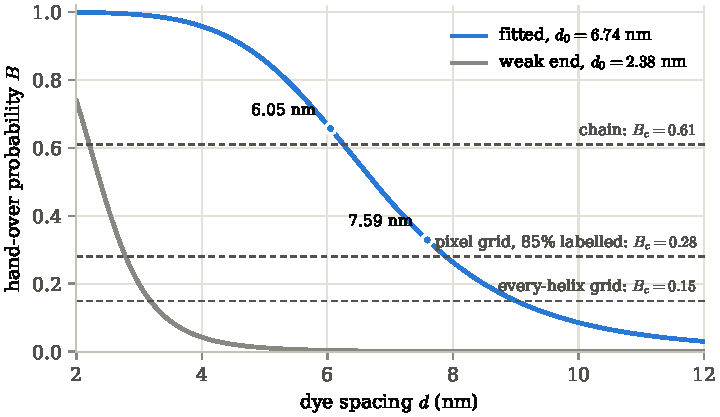
\includegraphics[width=0.82\linewidth]{fig_coupling.pdf}
\caption{Hand-over probability $B=r/(1+r)$ against spacing for the fitted and
weak ends of the coupling. Dashed lines: critical values $B_c$ per nearest bond
from simulation (Sec.~4). Dots: the two origami grids under the fitted law.}
\label{fig:coupling}
\end{figure}

\section{Mapping onto the contact process}

With $\pb=0$ and no spontaneous recovery, the master equation is generated by
\begin{equation}
  n_i:\;1\to0 \text{ at rate } 1,
  \qquad
  n_i:\;0\to1 \text{ at rate } \sum_j r_{ij}\,n_j .
\end{equation}
This is the contact process with control parameter $r_1=r(a)$, $a$ the
nearest-neighbour distance. The state $n_i\equiv0$ is absorbing. Below a critical
$r_c$ activity dies; above it a finite density of ON dyes persists.

\subsection{Conditions of the DP conjecture}

Janssen and Grassberger conjectured that a continuous transition into a single
absorbing state, with short-range interactions, no additional symmetry or
conservation law, and no quenched disorder, belongs to the DP class. We check
each condition.

\paragraph{Single absorbing state.} Holds without spontaneous recovery.
Bleached sites are inert and do not create a second absorbing state.

\paragraph{Range of the interaction.} The coupling decays as $d^{-6}$. For DP
with long-range spreading $P(d)\propto d^{-(D+\sigma)}$, the long-range term is
irrelevant when $\sigma$ exceeds a threshold close to 2 in the dimensions of
interest. In $D=2$, $D+\sigma=6$ gives $\sigma=4$. F\"orster coupling is
therefore short-range for the purposes of DP.

\paragraph{No extra symmetry or conservation.} The rules conserve nothing and
have no particle--hole or parity symmetry.

\paragraph{Non-additive rates.} When several dark neighbours surround an ON dye,
they compete for the same excitation through the denominator of $E_{ij}$. The
wake rates are then sublinear in the number of dark neighbours. In addition,
excitations lost to transfer are not available for switching off, so an ON dye
with many dark neighbours lives longer. At $d=\SI{6}{nm}$ a single neighbour
takes about 11\,\% of the excitations and four take about 45\,\%. These are
local, state-dependent rates that preserve the absorbing state; they shift
$r_c$ but leave the universality class unchanged.

\paragraph{Quenched disorder.} Fails in principle; see Sec.~\ref{sec:disorder}.

\subsection{Exponents}

We use the standard $2+1$-dimensional DP values:
\begin{center}
\begin{tabular}{lll}
\toprule
Exponent & Value & Defined by\\
\midrule
$\beta$ & 0.583 & $\rho_{\mathrm{st}}\sim(r-r_c)^\beta$\\
$\nperp$ & 0.733 & $\xi_\perp\sim|r-r_c|^{-\nperp}$\\
$\npar$ & 1.295 & $\xi_\parallel\sim|r-r_c|^{-\npar}$\\
$\delta=\beta/\npar$ & 0.4505 & $\rho(t)\sim t^{-\delta}$ at $r_c$, from a fully active start\\
$\sigma$ & 2.18 & field exponent, $\rho_{\mathrm{st}}(r_c,h)\sim h^{\beta/\sigma}$\\
\bottomrule
\end{tabular}
\end{center}

\section{Perturbations of the DP fixed point}

Each imperfection is a relevant perturbation. At criticality, it is invisible at
short times and takes over after a crossover time that scales as a power of its
strength. That time is the length of the observable critical window
(Fig.~\ref{fig:window}).

\begin{figure}[h]
\centering
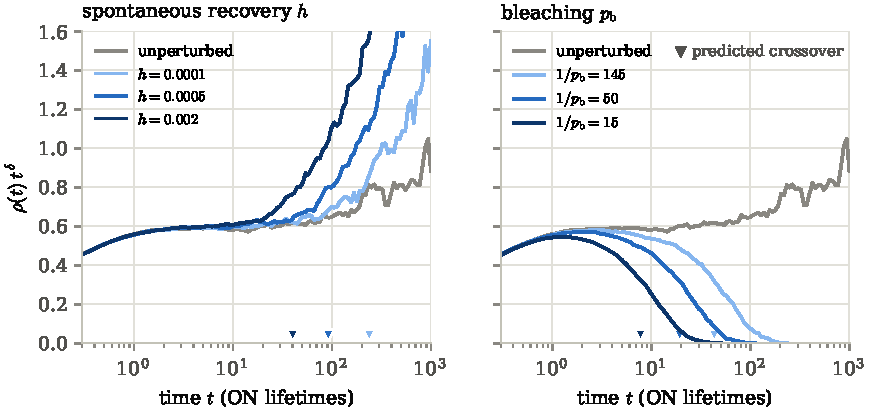
\includegraphics[width=\linewidth]{fig_window.pdf}
\caption{Critical decay at the threshold of the pixel grid ($r_1=0.334$,
$256\times256$ sites, two runs each), scaled by $t^{\delta}$ so that pure DP is
flat. Spontaneous recovery bends the curve up, bleaching bends it down.
Triangles: crossover times predicted by Eqs.~(\ref{eq:th}) and (\ref{eq:tb})
with unit prefactor.}
\label{fig:window}
\end{figure}

\subsection{Spontaneous recovery as the conjugate field}

Dark dyes recover on their own at rate $h$ (per ON lifetime), giving the extra
transition $n_i:0\to1$ at rate $h$. This is the field conjugate to the order
parameter in DP. At $r=r_c$ the scaling form
\begin{equation}
  \rho(t,h) = t^{-\delta}\, F\!\left(h\, t^{\sigma/\npar}\right)
\end{equation}
gives a crossover when $h\,t^{\sigma/\npar}\sim1$:
\begin{equation}
  \boxed{\;t_h \sim h^{-\npar/\sigma} = h^{-0.59}\;}
  \label{eq:th}
\end{equation}

\subsection{Photobleaching as activity-driven dilution}

Each ON period removes a dye with probability $\pb$, so the density of live dyes
$c(t)$ obeys
\begin{equation}
  \dot c = -\pb\,\rho(t).
\end{equation}
A lower site density lowers the effective coupling, which acts as a shift of the
control parameter proportional to the accumulated activity:
\begin{equation}
  \Delta(t)\;\propto\;\pb\int_0^t\rho(t')\,dt' \;\sim\; \pb\, t^{1-\delta},
\end{equation}
using $\rho\sim t^{-\delta}$ at criticality. The shift becomes comparable to the
distance from criticality probed at time $t$, $t^{-1/\npar}$, when
$\pb\,t^{1-\delta+1/\npar}\sim1$:
\begin{equation}
  \boxed{\;t_b \sim \pb^{-1/(1-\delta+1/\npar)} = \pb^{-0.76}\;}
  \label{eq:tb}
\end{equation}
The exponent is larger than in Eq.~\eqref{eq:th}, so for comparable strengths
bleaching ends the critical window first. This is the immunisation-type
perturbation studied by Jim\'enez-Dalmaroni and Hinrichsen (2003), in which
reinfection differs from first infection and the DP fixed point is unstable.

\subsection{Quenched disorder}\label{sec:disorder}

Missing dyes, frozen position errors and frozen dipole orientations make the
couplings $r_{ij}$ random but fixed in time. By the Harris criterion, such
disorder is relevant at the DP fixed point if
\begin{equation}
  D\,\nperp < 2 .
\end{equation}
In $D=2$, $D\nperp=1.47$, so disorder is relevant. For strong disorder the
transition flows to an infinite-randomness fixed point with activated scaling
and a Griffiths region (Vojta, Farquhar and Mast 2009). For weak disorder the
crossover length is large, and bleaching ends the critical window first.

Three sources of disorder are specific to the dye lattice:
\begin{itemize}
  \item \emph{Missing dyes.} Staple incorporation is about 84\,\%; vacancies
  raise $r_c$ approximately in proportion to $1/c$.
  \item \emph{Spacing errors.} Through $\delta r/r=-6\,\delta d/d$, a
  \SI{1}{nm} error at \SI{6}{nm} changes a bond by about 100\,\%. Because the
  coupling is convex in $d$, averaging over spacing errors raises the mean
  coupling.
  \item \emph{Orientation factor.} Eq.~\eqref{eq:forster} contains $\kappa^2$.
  If the dyes rotate freely within the excited-state lifetime, $\kappa^2=2/3$
  for every bond. If they are frozen (Cy5 partly stacks on DNA), $\kappa^2$
  varies between 0 and 4 from bond to bond. This could be the largest source of
  disorder, and it is unmeasured.
\end{itemize}

\section{Comparison with simulation}

We simulated the rules of Sec.~2 exactly (Gillespie algorithm) on a
$256\times256$ pixel grid at its threshold, $r_1=0.334$, quenched from fully ON.
Table~\ref{tab:check} compares the time at which $\rho(t)$ departs from the
unperturbed critical decay with Eqs.~\eqref{eq:th} and \eqref{eq:tb}
(see also Fig.~\ref{fig:crossover}). The prefactors of the scaling forms are set
to 1; only the exponents are predicted.

\begin{figure}[h]
\centering
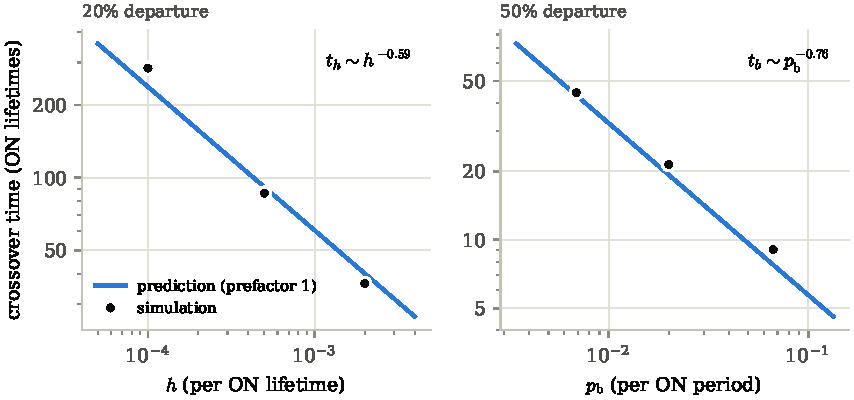
\includegraphics[width=\linewidth]{fig_crossover.pdf}
\caption{Crossover times against perturbation strength, log--log. Lines: the
scaling predictions with unit prefactor; points: simulation.}
\label{fig:crossover}
\end{figure}

\begin{table}[h]
\centering
\caption{Crossover times in ON lifetimes: scaling prediction against simulation.}
\label{tab:check}
\begin{tabular}{llcc}
\toprule
Perturbation & Strength & Predicted & Simulated\\
\midrule
Field, Eq.~\eqref{eq:th} & $h=0.002$  & 40  & 36 (20\,\% departure)\\
                         & $h=0.0005$ & 91  & 86\\
                         & $h=0.0001$ & 238 & 284\\
\midrule
Bleaching, Eq.~\eqref{eq:tb} & $1/\pb=15$  & 7.8 & 9.1 (50\,\% departure)\\
                             & $1/\pb=50$  & 19  & 21\\
                             & $1/\pb=145$ & 43  & 44\\
\bottomrule
\end{tabular}
\end{table}

The agreement in scaling across a factor of 20 in $h$ and 10 in $\pb$ supports
both the mapping to DP and the treatment of the perturbations. The absolute
agreement depends on the choice of departure threshold, which absorbs the
unknown prefactor.

\section{Consequences for an experiment}

\begin{enumerate}
  \item \textbf{Scaling of the crossover, not of the decay.} The critical decay
  itself is visible over about one decade, too little to extract $\delta$.
  The crossover times scale as $h^{-0.59}$ and $\pb^{-0.76}$, so varying
  the bleaching budget (oxygen scavenger, thiol) or the recovery rate and
  measuring the duration of the flash tests DP exponents without two decades of
  power law.
  \item \textbf{An independent field.} Weak \SI{405}{nm} illumination
  reactivates Cy5, tuning $h$ without changing $r$. pH changes $r$ through
  $\poff$; the two knobs together scan the $(r,h)$ plane.
  \item \textbf{What the pair experiment measures.} By Eq.~\eqref{eq:d0}, a pair
  measurement of $B(d)$ determines $\eta/\poff$, the single photophysical ratio
  that sets every coupling in the lattice.
  \item \textbf{Testing $\kappa^2$.} Comparing pairs with rigid and flexible
  linkers, or measuring dye anisotropy on origami, decides whether orientation
  disorder must be included.
\end{enumerate}

\section*{Caveats}
The weak-transfer limit is used in Eq.~\eqref{eq:d0}; at short range
($d\lesssim\SI{5}{nm}$) the full $E_{ij}$ must be kept. The bleaching argument
treats dilution as a uniform shift of the control parameter and ignores the
spatial correlation of bleached sites, which follow past activity. Dyes are
treated as two-state; triplet, \emph{cis} and radical intermediates are folded
into the rates.

\section*{References}
\begin{itemize}\small
  \item D.~A. Helmerich \emph{et al.}, Photoswitching fingerprint analysis
  bypasses the 10-nm resolution barrier, \emph{Nat.\ Methods} \textbf{19},
  986 (2022).
  \item V.~Ebert, M.~Sauer, S.~Doose, Energy transfer leaves fingerprints in
  cyanine photoswitching behavior, \emph{PLOS Comput.\ Biol.}\ (2026),
  doi:10.1371/journal.pcbi.1014322.
  \item H.~Hinrichsen, Non-equilibrium critical phenomena and phase transitions
  into absorbing states, \emph{Adv.\ Phys.}\ \textbf{49}, 815 (2000).
  \item A.~Jim\'enez-Dalmaroni, H.~Hinrichsen, Epidemic processes with
  immunization, \emph{Phys.\ Rev.\ E} \textbf{68}, 036103 (2003).
  \item T.~Vojta, A.~Farquhar, J.~Mast, Infinite-randomness critical point in
  the two-dimensional disordered contact process, \emph{Phys.\ Rev.\ E}
  \textbf{79}, 011111 (2009).
  \item K.~A. Takeuchi \emph{et al.}, Experimental realization of directed
  percolation criticality in turbulent liquid crystals, \emph{Phys.\ Rev.\ E}
  \textbf{80}, 051116 (2009).
\end{itemize}

\end{document}
